\documentclass[a4paper]{article}

\usepackage[english]{babel}
\usepackage[utf8]{inputenc}
\usepackage{listings}
\usepackage{amsmath}

\usepackage{dcolumn}
\usepackage{booktabs}
\usepackage{tikz}
\usepackage{graphicx}

\usetikzlibrary{positioning,shapes,arrows}

\newcolumntype{M}[1]{D{.}{.}{1.#1}}


\title{Exercise Sheet 2}
\begin{document}
\maketitle

\section*{Problem 2.1}
a)

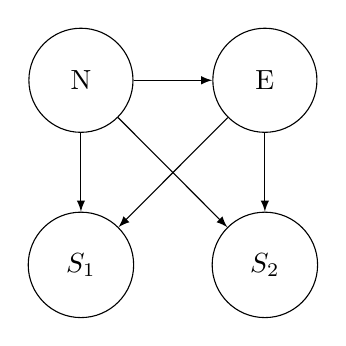
\begin{tikzpicture}[
  node distance=1cm and 1cm,
  mynode/.style={draw,circle,text width=1cm,align=center}
]
\node[mynode] (n) {N};
\node[mynode,right=of n] (e) {E};
\node[mynode,below=of n] (s1) {$S_1$};
\node[mynode,below=of e] (s2) {$S_2$};

\path (n) edge[-latex] (s1)
(n) edge[-latex] (e)
(n) edge[-latex] (s2)
(e) edge[-latex] (s1) 
(e) edge[-latex] (s2);
\end{tikzpicture}
It is assumed that nuclear test might cause earthquakes (so there must be a path from $N$ to $E$). Nuclear tests and earthquakes might cause the seismometeres to raise an alarm (so paths from $N$/$E$ to $S_1$/$S_2$).

\noindent\\
b)

\begin{tikzpicture}[
  node distance=1cm and 1cm,
  mynode/.style={draw,circle,text width=1cm,align=center}
]
\node[mynode] (s1) {$S_1$};
\node[mynode,right=of n] (s2) {$S_2$};
\node[mynode,below=of n] (e) {E};
\node[mynode,right=of e] (n) {N};

\path (s1) edge[-latex] (e)
(s1) edge[-latex] (n)
(s2) edge[-latex] (e) 
(s2) edge[-latex] (n);
\end{tikzpicture}
If the seismometers raise an alarm, the probabilities that there is an earthquake and/or a nuclear test are higher (so paths from $S_1$/$S_2$ to $E$/$N$). It is assumed that earthquakes don't influence the probability of nuclear tests.

\section*{Problem 2.2}

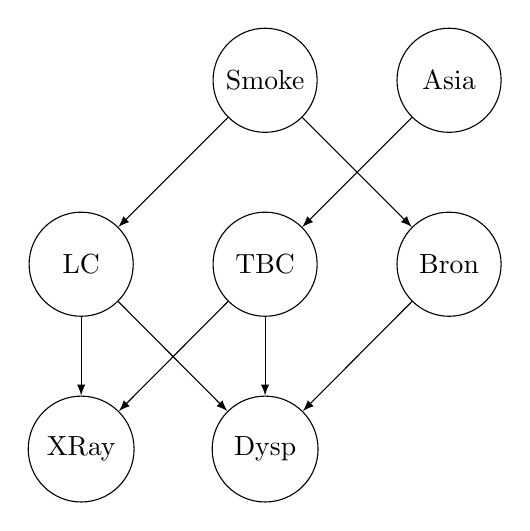
\begin{tikzpicture}[
  node distance=1cm and 1cm,
  mynode/.style={draw,circle,text width=1cm,align=center}
]
\node[mynode] (smoke) {Smoke};
\node[mynode,below = of smoke] (tbc) {TBC};
\node[mynode,right=of smoke] (asia) {Asia};
\node[mynode,left =of tbc] (lc) {LC};
\node[mynode,right = of tbc] (bron) {Bron};
\node[mynode,below = of lc] (xray) {XRay};
\node[mynode,below = of tbc] (dysp) {Dysp};

\path (smoke) edge[-latex] (lc)
(smoke) edge[-latex] (bron)
(asia) edge[-latex] (tbc)
(lc) edge[-latex] (xray)
(lc) edge[-latex] (dysp)
(tbc) edge[-latex] (xray)
(tbc) edge[-latex] (dysp)
(bron) edge[-latex] (dysp);
\end{tikzpicture}

\section*{Problem 2.3}
1.)

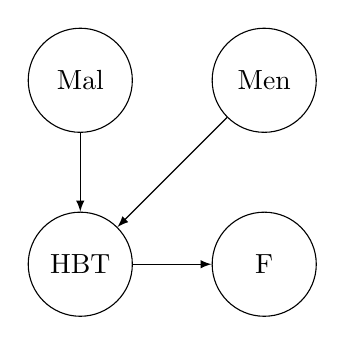
\begin{tikzpicture}[
  node distance=1cm and 1cm,
  mynode/.style={draw,circle,text width=1cm,align=center}
]
\node[mynode] (mal) {Mal};
\node[mynode,below = of mal] (hbt) {HBT};
\node[mynode,right=of mal] (men) {Men};
\node[mynode,below =of men] (f) {F};

\path (mal) edge[-latex] (hbt)
(men) edge[-latex] (hbt)
(hbt) edge[-latex] (f);

\end{tikzpicture}

Imagine a table left of the $HBT$ node and right of the $F$ node.

\includegraphics[scale=0.5]{alberteinstein1.jpg}

\newpage
\noindent
2.)
\begin{align*}
    P(mal, \lnot men | f) &= \frac{\sum_{hbt, f} P(mal, \lnot men, hbt, f)}{ \sum_{mal, men, hbt}P(mal, men, hbt, f)} \\
    &= \frac{\sum_{hbt, f} P(mal) \cdot P(\lnot men) \cdot P(hbt|mal, men) \cdot P(f|hbt)}{\sum_{mal, men, hbt}P(mal) \cdot P(men) \cdot P(hbt|mal, men) \cdot P(f|hbt)}\\
    &= \frac{\sum_{hbt, f} 0.04 \cdot P(hbt|mal, \lnot men) \cdot P(f|hbt)}{\sum_{mal, men, hbt} P(mal) \cdot P(men) \cdot P(hbt|mal, men) \cdot P(f|hbt)}\\
    &= \frac{0.04}{0.0009025 + 0.0000001 + 0.00342 + 0.0000008 + 0.16245 + 0.000038 + 0.00361 + 0.0000076}\\
    &= \frac{0.04}{0.170429} \approx 0.23470184064918529124
\end{align*}

\end{document}
